\section{Introduction}

Given a grammar $G$, the syntax analyzer reads a source string and: 
\begin{enumerate}
    \item If the string belongs to the language $L(G)$, then exhibits a derivation or builds a syntax tree of the string. 
    \item Otherwise, it stops and notifies the error, possibly with a diagnostic.
\end{enumerate}
If the source string is ambiguous, the result of the analysis is a set of derivations, also called forest of trees. 
Two analyzer classes exist, determined by whether the derivation is rightmost or leftmost, and by the reconstruction order of the derivation.
\begin{definition}[\textit{Bottom-up analysis}]
    The bottom-up analysis involves constructing the rightmost derivation in reverse order and analyzing the tree from leaves to root through reductions.
\end{definition}
\begin{definition}[\textit{Top-down analysis}]
    The top-down analysis involves constructing the leftmost derivation in direct order and analyzing the tree from root to leaves through expansions.
\end{definition}
\begin{example}
    Let's examine the string $aabbbaaaa$ generated by the grammar: 
    \[\begin{cases}
        S \rightarrow aSAB \\
        S \rightarrow b \\
        A \rightarrow bA \\
        B \rightarrow cB \\
        B \rightarrow a \\
    \end{cases}\]
    The tree resulting from the top-down analysis of the given string is depicted below, with numbering indicating the order of rule application:
    \begin{figure}[H]
        \centering
        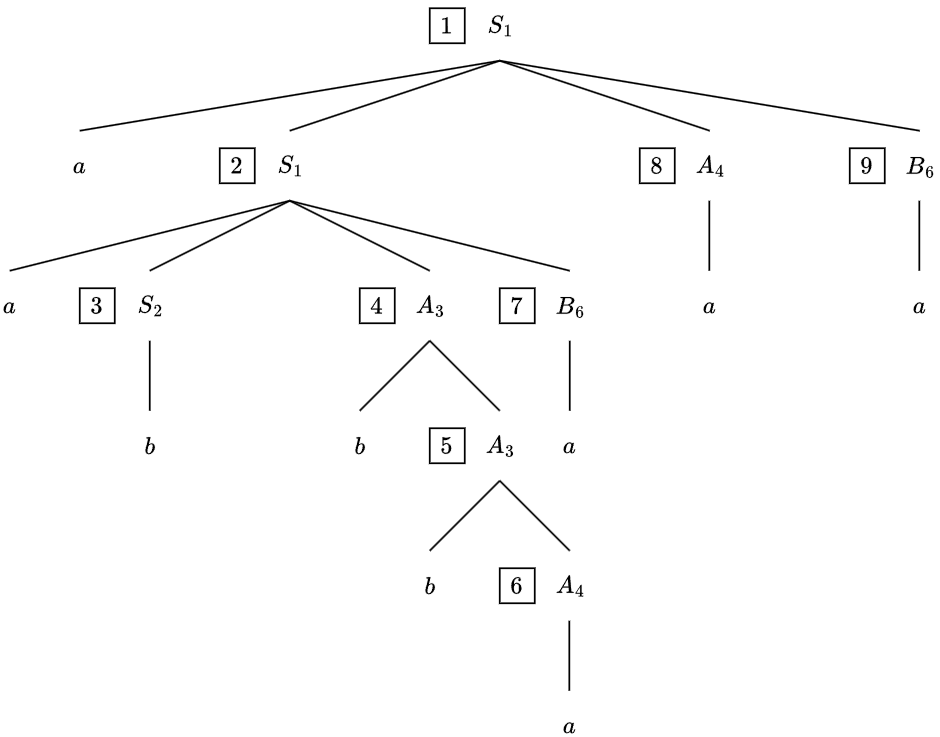
\includegraphics[width=0.75\linewidth]{images/tda.png}
    \end{figure}
    Similarly, the tree corresponding to the bottom-up analysis of the given string is illustrated below: 
    \begin{figure}[H]
        \centering
        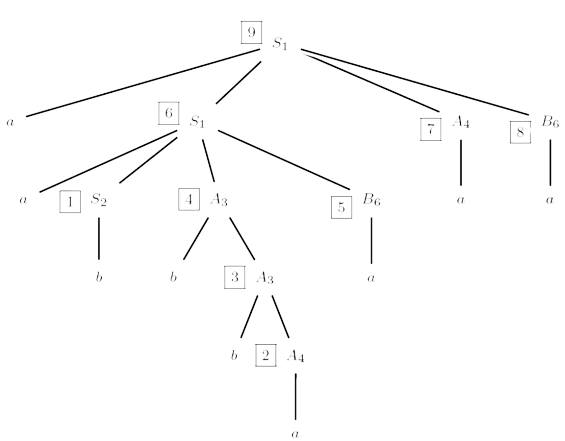
\includegraphics[width=0.75\linewidth]{images/bua.png}
    \end{figure}
\end{example}